\chapter{Compressible Flow Solver}

\section{Synopsis}
The CompressibleFlowSolver allows us to solve
the unsteady compressible Euler and Navier-Stokes 
equations for 1D/2D/3D problems using a discontinuous 
representation of the variables. In the following we describe 
both the compressible Euler and the Navier-Stokes equations.

\subsection{Euler equations}
The Euler equations can be expressed as a hyperbolic 
conservation law in the form 
\begin{equation}\label{eq:euler}
\frac{\partial \mathbf{q} }{\partial t} + \frac{\partial \mathbf{f}_i}{\partial x} 
+ \frac{\partial \mathbf{g}_i}{\partial y} +  
\frac{\partial \mathbf{h}_i}{\partial z} = 0,
\end{equation}
where $\mathbf{q} $ is the vector of the conserved variables, 
$\mathbf{f}_i =  \mathbf{f}_i (\mathbf{q})$, $\mathbf{g}_i 
= \mathbf{g}_i (\mathbf{q})$ and $\mathbf{h}_i = 
\mathbf{h}_i (\mathbf{q})$ are  the vectors of the 
inviscid fluxes
\begin{equation}
\mathbf{q} =\left\{
\begin{array}{c}
\rho \\
\rho u \\
\rho v \\ 
\rho w \\
E
\end{array} \right\}, \hspace{0.5 cm}
\mathbf{f}_i =\left\{
\begin{array}{c}
\rho u \\
p + \rho u^2 \\
\rho u v \\ 
\rho u w \\
u (E + p)
\end{array} \right\}, \hspace{0.5 cm}
\mathbf{g}_i =\left\{
\begin{array}{c}
\rho v \\
\rho u v \\
p + \rho v^2 \\ 
\rho v w \\
v (E + p)
\end{array} \right\}, \hspace{0.5 cm}
\mathbf{h}_i =\left\{
\begin{array}{c}
\rho w \\
\rho u w \\
\rho v w \\ 
p + \rho w^2 \\
w (E + p)
\end{array} \right\},
\label{Euler}
\end{equation}
where $\rho$ is the density, $u$, $v$ and $w$ are the velocity components in $x$, $y$ and 
$z$ directions, $p$ is the pressure and $E$ is the total energy. In this work we considered 
a perfect gas law for which the pressure is related to the total energy by the following expression
\begin{equation}
E = \frac{p}{\gamma - 1} + \frac{1}{2} \rho(u^2 + v^2 + w^2), 
\label{energy}
\end{equation}
where $\gamma$ is the ratio of specific heats.
\subsection{Compressible Navier-Stokes equations}
The Navier-Stokes equations include the effects of fluid viscosity and heat 
conduction and are consequently composed by an inviscid and a viscous 
flux. They depend not only on the conserved variables but also, indirectly, 
on their gradient. The second order partial differential equations for the 
three-dimensional case can be written as:
\begin{equation}
\frac{\partial \mathbf{q} }{\partial t} + 
\frac{\partial \mathbf{f}}{\partial x} + 
\frac{\partial \mathbf{g}}{\partial y} +  
\frac{\partial \mathbf{h}}{\partial z} = 0,
\end{equation}
where $\mathbf{q} $ is the vector of the conserved variables, $\mathbf{f} = 
\mathbf{f} (\mathbf{q}, \nabla (\mathbf{q}))$, 
$\mathbf{g}=  \mathbf{g} (\mathbf{q}, \nabla (\mathbf{q}))$ and $\mathbf{h} = 
\mathbf{h} (\mathbf{q}, \nabla (\mathbf{q}))$ 
are the vectors of the  fluxes which can also be written as:
\begin{equation}
\begin{array}{l}
\mathbf{f} = \mathbf{f}_i - \mathbf{f}_v,
\mathbf{g} = \mathbf{g}_i - \mathbf{g}_v,
\mathbf{h} = \mathbf{h}_i - \mathbf{h}_v, 
\end{array}
\end{equation}
where $\mathbf{f}_i$, $\mathbf{g}_i $ and $\mathbf{h}_i$ are the inviscid fluxes 
of Eq. (\ref{Euler}) and $\mathbf{f}_v$, $\mathbf{g}_v $ and $\mathbf{h}_v$ are 
the viscous fluxes which take the following form:
\begin{equation}
\begin{array}{c} \vspace{0.2 cm}
\mathbf{f}_v =\left\{
\begin{array}{c}
0 \\
\tau_{xx} \\
\tau_{yx} \\ 
\tau_{zx} \\
u \tau_{xx} + v \tau_{yx} + w \tau_{zx} + k T_x
\end{array} \right\},  \hspace{0.2 cm}
\mathbf{g}_v =\left\{
\begin{array}{c}
0 \\
\tau_{xy} \\
\tau_{yy} \\ 
\tau_{zy} \\
u \tau_{xy} + v \tau_{yy} + w \tau_{zy} + k T_y
\end{array} \right\}, \\ \vspace{0.2 cm}
\mathbf{h}_v =\left\{
\begin{array}{c}
0 \\
\tau_{xz} \\
\tau_{yz} \\ 
\tau_{zz} \\
u \tau_{xz} + v \tau_{yz} + w \tau_{zz} + k T_z
\end{array} \right\},
\end{array} 
\label{viscous flux}
\end{equation}
where $\tau_{xx}$, $\tau_{xy}$, $\tau_{xz}$, $\tau_{yx}$, $\tau_{yx}$, 
$\tau_{yy}$, $\tau_{yz}$, $\tau_{zx}$, $\tau_{zy}$ and $\tau_{zz}$ are 
the components of the stress tensor\footnote{Note that we use Stokes 
hypothesis $\lambda = -2/3$.} 
\begin{equation}
\begin{array}{cc} \vspace{0.2 cm}
\tau_{xx} = 2 \mu \left( u_x - \frac{u_x + v_y + w_z}{3}  \right), &  \tau_{yy} = 
2 \mu \left( v_y - \frac{u_x + v_y + w_z}{3}  \right), \\  
\vspace{0.2 cm}\tau_{zz} = 2 \mu \left( w_z - \frac{u_x + v_y + w_z}{3}  \right), 
& \tau_{xy} = \tau_{yx} = \mu(v_x + u_y), \\  
\vspace{0.2 cm} \tau_{yz} = \tau_{zy} = \mu(w_y + v_z),  & \tau_{zx} = \tau_{xz} = 
\mu(u_z + w_x). \\
\end{array}
\end{equation}
where $\mu$ is the dynamic viscosity calculated using 
the Sutherland's law and $k$ is the thermal conductivity.

\subsection{Numerical discretisation}
In Nektar++ the spatial discretisation of the Euler and of the Navier-Stokes 
equations is projected in the polynomial space via a discontinuous projection.
Specifically we make use either of the discontinuous Galerkin (DG) method 
or the Flux Reconstruction (FR) approach. 
In both the approaches the physical domain $\Omega$ is divided into a mesh 
of $N$ non-overlapping elements $\Omega_{e}$ and the solution is allowed 
to be discontinuous at the boundary between two adjacent elements. 
Since the Euler as well as the Navier-Stokes equations are defined locally 
(on each element of the computational domain), it is necessary to define 
a term to couple the elements of the spatial discretisation in order to allow 
information to propagate across the domain. This term, called numerical 
interface flux, naturally arises from the discontinuous Galerkin formulation 
as well as from the Flux Reconstruction approach. 

For the advection term it is common to solve a Riemann problem at each 
interface of the computational domain through exact or approximated Riemann
solvers. In Nektar++ there are different Riemann solvers, one exact and nine 
approximated. The exact Riemann solver applies an iterative procedure to 
satisfy conservation of mass, momentum and energy and the equation of 
state. The left and right states are connected either with the unknown variables 
through the Rankine-Hugoniot relations, in the case of shock, or the isentropic 
characteristic equations, in the case of rarefaction waves. Across the contact 
surface, conditions of continuity of pressure and velocity are employed. 
Using these equations the system can be reduced to a non-linear algebraic 
equation in one unknown (the velocity in the intermediate state) that is solved 
iteratively using a Newton method. Since the exact Riemann solver gives 
a solution with an order of accuracy that is related to the residual in the 
Newton method, the accuracy of the method may come at high computational 
cost. The approximated Riemann solvers are simplifications of the exact solver.

Concerning the diffusion term, the coupling between the elements is achieved 
by using a local discontinuous Galerkin (LDG) approach as well as five different 
FR diffusion terms.

The boundary conditions are also implemented by exploiting the numerical
interface fluxes just mentioned. 
For a more detailed description of the above the interested reader can refer 
to \cite{DeGMen14} and \cite{MenDeG14}.

\section{Usage}
\begin{lstlisting}[style=BashInputStyle]
CompressibleFlowSolver session.xml
\end{lstlisting}


\section{Session file configuration}
In the following we describe the session file configuration. Specifically we consider the
sections under the tag \inltt{<CONDITIONS>} in the session (.xml) file.
\subsection*{Parameters}
Under this section it is possible to set the parameters of the simulation.
\begin{lstlisting}[style=XmlStyle]
<PARAMETERS>
  <P> TimeStep            = 0.0000001                  </P>
  <P> FinTime             = 1.0                        </P>
  <P> NumSteps            = FinTime/TimeStep           </P>
  <P> IO_CheckSteps       = 5000                       </P>
  <P> IO_InfoSteps        = 1                          </P>
  <P> Gamma               = 1.4                        </P>
  <P> pInf                = 101325                     </P>
  <P> rhoInf              = 1.225                      </P>
  <P> TInf                = pInf/(287.058*rhoInf)      </P>
  <P> Twall               = pInf/(287.058*rhoInf)+15.0 </P>
  <P> uInf                = 147.4                      </P>
  <P> vInf                = 0.0                        </P>
  <P> wInf                = 0.0                        </P>
  <P> mu                  = 1e-5                       </P>
  <P> Pr                  = 0.72                       </P>
  <P> thermalConductivity = 0.02                       </P>
</PARAMETERS>
\end{lstlisting}
\begin{itemize}
\item \inltt{TimeStep} is the time-step we want to use;
\item \inltt{FinTime} is the final physical time at which we want our simulation to stop;
\item \inltt{NumSteps} is the equivalent of \inltt{FinTime} but instead of specifying the 
physical final time we specify the number of time-steps;
\item \inltt{IO\_CheckSteps} sets the number of steps between successive checkpoint files;
\item \inltt{IO\_InfoSteps} sets the number of steps between successive info stats are printed 
to screen;
\item \inltt{Gamma} ratio of the specific heats. Default value = 1.4;
\item \inltt{pInf} farfield pressure (i.e. $p_{\infty}$). Default value = 101325 $Pa$;
\item \inltt{rhoInf} farfield density (i.e. $\rho_{\infty}$). Default value = 1.225 $Kg/m^{3}$;
\item \inltt{TInf} farfield temperature (i.e. $T_{\infty}$). Default value = 288.15 $K$;
\item \inltt{Twall} temperature at the wall when isothermal boundary 
conditions are employed (i.e. $T_{w}$). Default value = 300.15$K$;
\item \inltt{uint} farfield $X$-component of the velocity (i.e. $u_{\infty}$). Default value = 0.1 $m/s$;
\item \inltt{vInf} farfield $Y$-component of the velocity (i.e. $v_{\infty}$). Default value = 0.0 $m/s$;
\item \inltt{wInf} farfield $Z$-component of the velocity (i.e. $w_{\infty}$). Default value = 0.0 $m/s$;
\item \inltt{mu} dynamic viscosity (i.e. $\mu_{\infty}$). Default value = 1.78e-05 $Pa s$;
\item \inltt{Pr} Prandtl number. Default value = 0.72;
\item \inltt{thermalConductivity} thermal conductivity (i.e. $\kappa_{\infty}$). Default value = 0.0257 $W / (K m)$;
\end{itemize}

\subsection*{Solver info}
Under this section it is possible to set the solver information.
\begin{lstlisting}[style=XmlStyle]       
<SOLVERINFO>
  <I PROPERTY="EQType"                VALUE="NavierStokesCFE"     />
  <I PROPERTY="Projection"            VALUE="DisContinuous"       />
  <I PROPERTY="AdvectionType"         VALUE="WeakDG"              />
  <I PROPERTY="DiffusionType"         VALUE="LDGNS"               />
  <I PROPERTY="TimeIntegrationMethod" VALUE="ClassicalRungeKutta4"/>
  <I PROPERTY="UpwindType"            VALUE="ExactToro"           />
  <I PROPERTY="ProblemType"           VALUE="General"             />
  <I PROPERTY="ViscosityType"         VALUE="Constant"            />
</SOLVERINFO>
\end{lstlisting}
\begin{itemize}
\item \inltt{EQType} is the tag which specify the equations we want solve:
\begin{itemize}
\item \inltt{NavierStokesCFE} (Compressible Navier-Stokes equations);
\item \inltt{EulerCFE} (Compressible Euler equations).
\end{itemize}
\item \inltt{Projection} is the type of projection we want to use:
\begin{itemize}
\item \inltt{DisContinuous}.\\
Note that the Continuous projection is not supported in the Compressible Flow Solver. 
\end{itemize}
\item \inltt{AdvectionType} is the advection operator we want to use:
\begin{itemize}
\item \inltt{WeakDG} (classical DG in weak form);
\item \inltt{FRDG} (Flux-Reconstruction recovering nodal DG scheme);
\item \inltt{FRSD} (Flux-Reconstruction recovering a spectral difference (SD) scheme);
\item \inltt{FRHU} (Flux-Reconstruction recovering Huynh (G2) scheme);
\item \inltt{FRcmin} (Flux-Reconstruction with $c = c_{min}$);
\item \inltt{FRcinf} (Flux-Reconstruction with $c = \infty$).
\end{itemize}
\item \inltt{DiffusionType} is the diffusion operator we want to use:
\begin{itemize}
\item \inltt{WeakDG} (classical DG in weak form);
\item \inltt{FRDG} (Flux-Reconstruction recovering nodal DG scheme);
\item \inltt{FRSD} (Flux-Reconstruction recovering a spectral difference (SD) scheme);
\item \inltt{FRHU} (Flux-Reconstruction recovering Huynh (G2) scheme);
\item \inltt{FRcmin} (Flux-Reconstruction with $c = c_{min}$);
\item \inltt{FRcinf} (Flux-Reconstruction with $c = \infty$).
\end{itemize}
\item \inltt{TimeIntegrationMethod} is the time-integration scheme we want to use. 
Note that only an explicit discretisation is supported:
\begin{itemize}
\item \inltt{ForwardEuler};
\item \inltt{RungeKutta2\_ImprovedEuler};
\item \inltt{ClassicalRungeKutta4}.
\end{itemize}
\item \inltt{UpwindType} is the numerical interface flux (i.e. Riemann solver) 
we want to use for the advection operator:
\begin{itemize}
\item \inltt{AUSM0};
\item \inltt{AUSM1}; 
\item \inltt{AUSM2}; 
\item \inltt{AUSM3}; 
\item \inltt{Average}; 
\item \inltt{ExactToro};
\item \inltt{HLL};
\item \inltt{HLLC};
\item \inltt{LaxFriedrichs};
\item \inltt{Roe}.
\end{itemize}
\item \inltt{ProblemType} is the problem type we want to solve. 
This tag is supported for solving ad hoc problems such as the 
isentropic vortex or the Ringleb flow.
\begin{itemize}
\item \inltt{General};
\item \inltt{IsentropicVortex};
\item \inltt{RinglebFlow};\\[0.2em]
\end{itemize}
\item \inltt{ViscosityType} is the viscosity type we want to use:
\begin{itemize}
\item \inltt{Constant} (Constant viscosity);
\item \inltt{Variable} (Variable viscosity through the Sutherland's law.);
\end{itemize}
\end{itemize}

\subsection*{Boundary conditions}
In this section we can specify the boundary conditions for our problem.
First we need to define the variables under the section \inltt{VARIABLES}.
For a 1D problem we have:
\begin{lstlisting}[style=XmlStyle]        
<VARIABLES>
  <V ID="0"> rho  </V>
  <V ID="1"> rhou </V>
  <V ID="4"> E    </V>
</VARIABLES>
\end{lstlisting}

For a 2D problem we have
\begin{lstlisting}[style=XmlStyle]        
<VARIABLES>
  <V ID="0"> rho  </V>
  <V ID="1"> rhou </V>
  <V ID="2"> rhov </V>
  <V ID="4"> E    </V>
</VARIABLES>
\end{lstlisting}

For a 3D problem we have:
\begin{lstlisting}[style=XmlStyle]        
<VARIABLES>
  <V ID="0"> rho  </V>
  <V ID="1"> rhou </V>
  <V ID="2"> rhov </V>
  <V ID="3"> rhow </V>
  <V ID="4"> E    </V>
</VARIABLES>
\end{lstlisting}

After having defined the variables depending on the dimensions of the problem we want to solve
it is necessary to specify the boundary regions on which we want to define the boundary conditions:
\begin{lstlisting}[style=XmlStyle]        
<BOUNDARYREGIONS>
  <B ID="0"> C[100] </B>
</BOUNDARYREGIONS>
\end{lstlisting}

Finally we can specify the boundary conditions on the regions specified under \inltt{BOUNDARYREGIONS}.
In the following some examples for a 2D problem:
\begin{itemize}
\item Slip wall boundary conditions:
\begin{lstlisting}[style=XmlStyle]                
<BOUNDARYCONDITIONS>
  <REGION REF="0">
    <D VAR="rho"  USERDEFINEDTYPE="Wall" VALUE="0" />
    <D VAR="rhou" USERDEFINEDTYPE="Wall" VALUE="0" />
    <D VAR="rhov" USERDEFINEDTYPE="Wall" VALUE="0" />
    <D VAR="E"    USERDEFINEDTYPE="Wall" VALUE="0" />
  </REGION>
</BOUNDARYCONDITIONS>
\end{lstlisting}

\item No-slip wall boundary conditions:
\begin{lstlisting}[style=XmlStyle]                
<BOUNDARYCONDITIONS>
  <REGION REF="0">
    <D VAR="rho"  USERDEFINEDTYPE="WallViscous" VALUE="0" />
    <D VAR="rhou" USERDEFINEDTYPE="WallViscous" VALUE="0" />
    <D VAR="rhov" USERDEFINEDTYPE="WallViscous" VALUE="0" />
    <D VAR="E"    USERDEFINEDTYPE="WallViscous" VALUE="0" />
  </REGION>
</BOUNDARYCONDITIONS>
\end{lstlisting}

\item Farfield boundary conditions (including inviscid characteristic boundary conditions):
\begin{lstlisting}[style=XmlStyle] 
<BOUNDARYCONDITIONS>  
  <REGION REF="0">
    <D VAR="rho"  VALUE="rhoInf" />
    <D VAR="rhou" VALUE="rhoInf*uInf" />
    <D VAR="rhov" VALUE="rhoInf*vInf" />
    <D VAR="E"    
    VALUE="pInf/(Gamma-1)+0.5*rhoInf*(uInf*uInf+vInf*vInf+wInf*wInf)"/>
  </REGION>
</BOUNDARYCONDITIONS>
\end{lstlisting}

\item Pressure outflow boundary conditions:
\begin{lstlisting}[style=XmlStyle]                
<BOUNDARYCONDITIONS>
  <REGION REF="0">
    <D VAR="rho"  USERDEFINEDTYPE="PressureOutflow" VALUE="0" />
    <D VAR="rhou" USERDEFINEDTYPE="PressureOutflow" VALUE="0" />
    <D VAR="rhov" USERDEFINEDTYPE="PressureOutflow" VALUE="0" />
    <D VAR="E"    USERDEFINEDTYPE="PressureOutflow" VALUE="0" />
  </REGION>
</BOUNDARYCONDITIONS>
\end{lstlisting}
\end{itemize}

\subsection*{Initial conditions and exact solution}
Under the two following sections it is possible to define the initial conditions and the exact solution (if existent).
\begin{lstlisting}[style=XmlStyle]           
<FUNCTION NAME="InitialConditions">
  <E VAR="rho"    VALUE="rhoInf"/>
  <E VAR="rhou"   VALUE="rhoInf*uInf"   />
  <E VAR="rhov"   VALUE="rhoInf*vInf"   />
  <E VAR="E"      
  VALUE="pInf/(Gamma-1)+0.5*rhoInf*(uInf*uInf+vInf*vInf+wInf*wInf)"/>
</FUNCTION>
                
<FUNCTION NAME="ExactSolution">
  <E VAR="rho"    VALUE="rhoInf"          />
  <E VAR="rhou"   VALUE="rhoInf*uInf"   />
  <E VAR="rhov"   VALUE="rhoInf*vInf"   />
  <E VAR="E"      
  VALUE="pInf/(Gamma-1)+0.5*rhoInf*(uInf*uInf+vInf*vInf+wInf*wInf)"/>
</FUNCTION>
\end{lstlisting}

\section{Examples}
\subsection{Shock capturing}
Compressible flow is characterised by abrupt changes in density within the flow domain often referred to as shocks. These discontinuities lead to numerical instabilities (Gibbs phenomena). This problem is prevented by locally adding a diffusion term to the equations to damp the numerical fluctuations. These fluctuations in an element are identified using a sensor algorithm which quantifies the smoothness of the solution within an element. The value of the sensor in an element is defined as
\begin{equation}\label{eq:sensor}
S_e=\frac{||\rho^p_e-\rho^{p-1}_e||_{L_2}}{||\rho_e^p||_{L_2}}
\end{equation}
An artificial diffusion term is introduced locally to the Euler equations to deal with flow discontinuity and the consequential numerical oscillations. Two models are implemented, a non-smooth and a smooth artificial viscosity model. 
\subsubsection{Non-smooth artificial viscosity model}
For the non-smooth artificial viscosity model the added artificial viscosity is constant in each element and discontinuous between the elements. The Euler system is augmented by an added laplacian term on right hand side of equation \ref{eq:euler}. The diffusivity of the system is controlled by a variable viscosity coefficient $\epsilon$. The value of $\epsilon$ is dependent on $\epsilon_0$, which is the maximum viscosity that is dependent on the polynomial order ($p$), the mesh size ($h$) and the maximum wave speed and the local sensor value. Based on pre-defined sensor threshold values, the variable viscosity is set accordingly
\begin{equation}
   \epsilon
=\epsilon_0\left \{ \begin{array}{l}
    0\	\	\	\	\	\	\	\	\	\	\	\	\	\	\	\	\	\	\	\	\	\	\	\	\	\	\	\	\	\	\	\	\	 \mbox{if}\		\	 s_e<s_\kappa-\kappa\\  
    0.5\left(1+\sin{\frac{\pi\left(S_e-s_\kappa\right)}{2\kappa}}\right)\	\	\	\	\	\	\mbox{if}\		\	 s_\kappa-\kappa<S_e<s_\kappa+\kappa\\
    1\	\	\	\	\	\	\	\	\	\	\	\	\	\	\	\	\	\	\	\	\	\	\	\	\	\	\	\	\	\	\	\	\	 \mbox{if}\		\ s_e > s_\kappa+\kappa
      \end{array} 
    \right.
\end{equation}
\begin{figure}[!htbp]
\begin{center}
\includegraphics[width = 0.47 \textwidth]{Figures/Mach_P4.eps}
\includegraphics[width = 0.47 \textwidth]{Figures/ArtVisc_P4.eps}
\caption{(a) Steady state solution for $M=0.8$ flow at $\alpha = 1.25^\circ$ past a NACA 0012 profile, (b) Artificial viscosity ($\epsilon$) distribution}
\label{fig:}
\end{center}
\end{figure}
\subsubsection{Smooth artificial viscosity model}
For the smooth artificial viscosity model an extra PDE for the artificial viscosity is appended to the Euler system
\begin{equation}\label{eq:euler}\begin{split}
\frac{\partial \epsilon}{\partial t} &= \nabla\cdot \left(\nabla \epsilon\right) + \frac{1}{\tau}\left(\frac{h}{p}\lambda_{max}S_\kappa - \epsilon\right)\	\	\	\	\	\	\textrm{on}\	\	\	\	\	\	\	\Omega\\
\frac{\partial \epsilon}{\partial n} &= 0\	\	\	\	\	\	\	\	\	\	\	\	\	\	\	\	\	\	\	\	\	\	\	\	\	\	\	\	\	\	\	\	\	\	\	\	\	\	\	\	\	\	\	\textrm{on}\	\	\	\	\	\	\	\Gamma
\end{split}
\end{equation}
where $S_\kappa$ is a normalised sensor value and serves as a forcing term for the artificial viscosity. A smooth artificial viscosity distribution is obtained.\\
\\
To enable the smooth viscosity model, the following line has to be added to the \inltt{SOLVERINFO} section:
\begin{lstlisting}[style=XmlStyle]
 <SOLVERINFO>
<I PROPERTY="ShockCaptureType"      VALUE="Smooth"               />
 <SOLVERINFO>
\end{lstlisting}
Furthermore, the extra viscosity variable \inltt{eps} has to be added to the variable list:
\begin{lstlisting}[style=XmlStyle]        
<VARIABLES>
  <V ID="0"> rho  </V>
  <V ID="1"> rhou </V>
  <V ID="2"> rhov </V>
  <V ID="4"> E    </V>
  <V ID="5"> eps </V>
</VARIABLES>
\end{lstlisting}
A similar addition has to be made for the boundary conditions and initial conditions. The tests that have been run started with a uniform homogeneous boundary condition and initial condition.
The following parameters can be set in the xml session file:
\begin{lstlisting}[style=XmlStyle]
<PARAMETERS>
<P> Skappa 	 	= -1.3                     </P>
<P> Kappa 	 	= 0.2                      </P> 
<P> mu0 	 	= 1.0                      </P>
<P> FH 	 	 	= 3                        </P>
<P> FL 	 	 	= 0.01*FH                  </P>
<P> C1 	 	 	= 0.03                     </P>
<P> C2 		 	= 5/3*C1                   </P>
</PARAMETERS>
\end{lstlisting}
where for now \inltt{FH} and \inltt{FL} are used to tune which range of the sensor is used as a forcing term and \inltt{C1} and \inltt{C2} are fixed constants which can be played around with to make the model more diffusive or not. However these constants are generally fixed.
\subsection{Variable polynomial order}
A sensor based $p$-adaptive algorithm is implemented to optimise the computational cost and accuracy. 
The DG scheme allows one to use different polynomial orders since the fluxes over the elements are determined using a Riemann solver and there is now further coupling between the elements. Furthermore, the initial $p$-adaptive algorithm uses the same sensor as the shock capturing algorithm to identify the smoothness of the local solution so it rather straightforward to implement both algorithms at the same time.\\
\\
The polynomial order in each element can be adjusted based on the sensor value that is obtained. Initially, a converged solution is obtained after which the sensor in each element is calculated. Based on the determined sensor value and the pre-defined sensor thresholds, it is decided to increase, decrease or maintain the degree of the polynomial approximation in each element and a new converged solution is obtained.\\
\begin{equation}\label{eq:pswitch}
  p_e =\left \{ \begin{array}{l}
    p_e-1\	\	\ \mbox{if}\		\	 s_e>s_{ds}\\  
    p_e+1\	\	\ \mbox{if}\		\	 s_{sm }<s_e<s_{ds}\\
    p_e\	\	\	\	\	\	\	\	\	 \mbox{if}\		\ s_{fl}<s_e<s_{sm}\\
    p_e-1\	\	\ \mbox{if}\		\	 s_e<s_{fl}
    \end{array} 
    \right.
\end{equation}
For now, the threshold values $s_e$, $s_{ds}$, $s_{sm}$ and $s_{fl}$ are determined empirically by looking at the sensor distribution in the domain. Once these values are set, two .txt files are outputted, one that has the composites called VariablePComposites.txt and one with the expansions called VariablePExpansions.txt. These values have to copied into a new .xml file to create the adapted mesh.


